\documentclass[11pt,letterpaper,titlepage]{article}

\usepackage{geometry}
\geometry{left=2cm,right=2cm,top=2cm,bottom=3cm}

\usepackage{setspace}
\onehalfspacing

\usepackage{multicol}
\setlength{\columnsep}{3em}

\usepackage{booktabs}

\usepackage[table,x11names]{xcolor}

\usepackage{multirow}

\usepackage{pgfgantt}

\usepackage{listings}

\usepackage{xcolor}
\definecolor{vgreen}{RGB}{104,180,104}
\definecolor{vblue}{RGB}{49,49,255}
\definecolor{vorange}{RGB}{255,143,102}

\lstdefinestyle{C-style}
{
    language=C,
    basicstyle=\small\ttfamily,
    keywordstyle=\color{vblue},
    identifierstyle=\color{black},
    commentstyle=\color{vgreen},
    % numbers=left,
    numberstyle=\tiny\color{black},
    numbersep=11pt,
    tabsize=4,
    moredelim=*[s][\colorIndex]{[}{]},
    literate=*{:}{:}1
}

\lstdefinestyle{txt-style}
{
    basicstyle=\small\ttfamily,
    % numbers=left,
    numbersep=11pt,
    tabsize=4,
    moredelim=*[s][\colorIndex]{[}{]},
    literate=*{:}{:}1
}

\usepackage{tikz}
\usetikzlibrary{shapes.geometric, arrows, positioning, fit,calc}
\newcommand*\circled[1]{\tikz[baseline=(char.base)]{
            \node[shape=circle,draw,inner sep=1pt] (char) {#1};}}
            
\usepackage{hyperref}
\hypersetup{
    colorlinks,
    citecolor=black,
    filecolor=black,
    linkcolor=black,
    urlcolor=black
}

\usepackage{pifont}

\usepackage[toc,page]{appendix}

\pagestyle{empty}
\usepackage{tikz}
\usetikzlibrary{shapes.geometric, arrows}

\usetikzlibrary{mindmap,trees}
\usepackage{verbatim}

\usepackage{indentfirst}
\setlength{\parindent}{2em}

\usepackage{listings}

\usepackage{chngcntr}
\counterwithin{section}{part}
\renewcommand\thesection{\arabic{section}}

\usepackage{graphicx}

\usepackage{subcaption}

\usepackage{fancyhdr}

\pagestyle{fancy}
\lhead{}
\rhead{}
\lfoot{ECEN 749 Section 601 Lab 4}
\cfoot{\thepage}
\rfoot{@Lei Wang (Wilson)}
\renewcommand{\headrulewidth}{0pt}
\renewcommand{\headwidth}{\textwidth}
\renewcommand{\footrulewidth}{0.4pt}
\newcommand{\RomanNumeralCaps}[1]
    {\MakeUppercase{\romannumeral #1}}

\makeatletter
\newcommand*\@lbracket{[}
\newcommand*\@rbracket{]}
\newcommand*\@colon{:}
\newcommand*\colorIndex{%
    \edef\@temp{\the\lst@token}%
    \ifx\@temp\@lbracket \color{black}%
    \else\ifx\@temp\@rbracket \color{black}%
    \else\ifx\@temp\@colon \color{black}%
    \else \color{vorange}%
    \fi\fi\fi
}
\makeatother

\usepackage{trace}

\begin{document}

\begin{titlepage}
  \centering
	{\scshape\large Texas A\&M University \par}
	\vspace{1cm}
	{\scshape\Large Department of Electrical and Computer Engineering \par}
	\vspace{4cm}
    \vspace{0.5cm}
	{\huge\bfseries ECEN 749 Microprocessor System Design\par}
	\vspace{4cm}
	{\Large Lab 4 Report (Section 601)\par}
	\vspace{1cm}
	{\Large Student: Lei Wang (Wilson)\par}
	\vspace{1cm}
	{\Large UIN: 829009485\par}
	\vspace{1cm}
	{\Large Instructor: Dr. Paul V. Gratz\par}
	\vspace{4cm}
	\vfill

  % Bottom of the page
	{\large Submitted: February 18th, 2020 \par}

\end{titlepage}

\newpage

\tableofcontents{}

\newpage

\part{Introduction}

The purpose of the lab is to teach students how to run Linux on the ZYBO Z7-10 board. The process involves creating the block diagram design, generating the BOOT.bin file, compiling the Linux kernel, configuring the devicetree and making the ramdisk image. All the files generated are transferred to a micro-SD card and the FPGA board is configured to boot from the micro-SD card. Picocom is used to observe the output.

\part{Procedure}

\begin{enumerate}
    
    \item Create the \textbf{hardware layout}:
    
    \begin{enumerate}
        
        \item Create a Vivado project with ZYBO Z7-10 selected as the target board.
        
        \item Create a block design with \textbf{ZYNQ7 Processing System} added. Configure the processing system using the \textbf{ZYBO\_Z7\_B2.tcl} file available in the shared project directory.
        
        \item Run block automation.
        
        \item Enable only the following in \textbf{Peripheral I/O Pins} tab in \textbf{Re-customize IP} window by double clicking on the processing system: \textbf{SD 0}, \textbf{UART 1}, \textbf{TTC 0}.
        
        \item Copy and paste the directory that contains the multiply IP to the project directory.
        
        \item Click on \textbf{Project Settings} $\rightarrow$ \textbf{IP} $\rightarrow$ the green + sign and add the directory that is copied.
        
        \item Go back to the block design and add the multiply IP.
        
        \item Run connection automation and regenerate layout:
        
        \begin{figure}[ht]
            \centering
            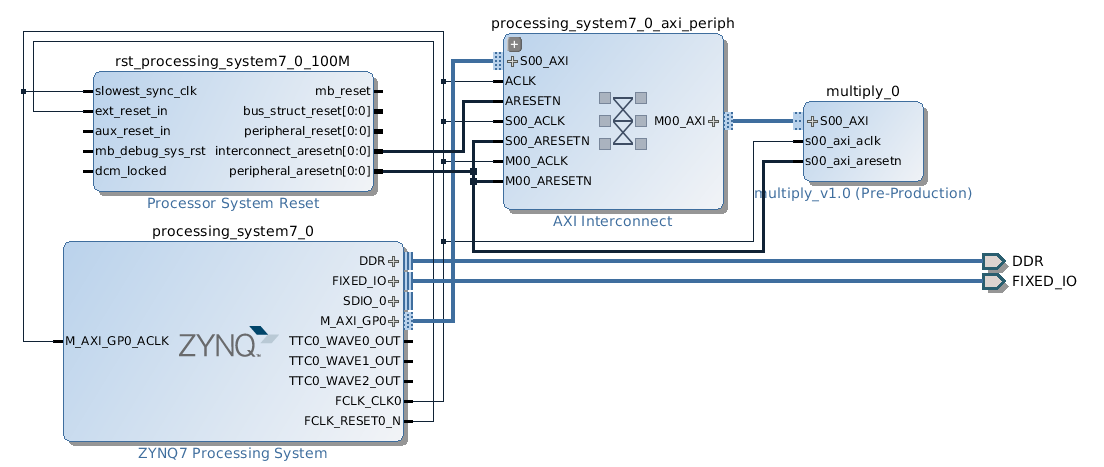
\includegraphics[width=0.8\textwidth]{block.png}
            \caption{Block design for lab 4.}
        \end{figure}
        
        \item Create HDL wrapper.
        
        \item Generate bitstream.
        
        \item Export hardware, including the bitstream.
        
    \end{enumerate}
    
    \item Create \textbf{u-boot}:
    
    \begin{enumerate}
        
        \item Use \verb|cp| command to copy \textbf{/mnt/lab\_files/ECEN449/u-boot.tar.gz} to the working directory of lab 4
        
        \item Run:
        
        \verb|tar -xvzf u-boot.tar.gz|
        
        Or:
        
        \verb|tar -xzf u-boot.tar.gz|
        
        If do not wish to see the verbose logging during the untar operation.
        
        \item Source the Vivado settings:
        
        \verb|source /opt/coe/Xilinx/Vivado/2015.2/settings64.sh|
        
        \item Change to the u-boot directory:
        
        \verb|cd u-boot|
        
        \item Configure u-boot to target at the ZYBO Z7-10 board by running:
        
        \verb|make CROSS_COMPILE=arm-xilinx-linux-gnueabi- zynq_zybo_config|
        
        \item Compile u-boot by running:
        
        \verb|make CROSS_COMPILE=arm-xilinx-linux-gnueabi-|
        
        \item Search in the u-boot directory for a file named \textbf{u-boot}. Add an \textbf{.elf} extension to the file name.
        
    \end{enumerate}
    
    \item Generate \textbf{BOOT.bin}:
    
    \begin{enumerate}
        
        \item Launch Xilinx SDK from Vivado.
        
        \item Create a new application project of type \textbf{First Stage Bootloader (FSBL)}. Name the project \textbf{FSBL}. Select \textbf{Zynq FSBL} as the template for the project.
        
        \item Right click on project \textbf{FSBL} $\rightarrow$ \textbf{Build Options} $\rightarrow$ \textbf{Build All}.
        
        \item Click on \textbf{Xilinx Tools} $\rightarrow$ \textbf{Create Zynq Boot Image}:
        
        \begin{table}[h!]
        \centering
        \begin{tabular}{@{}cllc@{}}
        \toprule
        Step & File Name              & Relative Path                                                  & Type       \\ \midrule
        1    & FSBL.elf               & \verb|.sdk/FSBL/Debug|                          & bootloader \\ \midrule
        2    & design\_1\_wrapper.bit & \verb|.sdk/design\_1\_wrapper\_hw\_platform\_0| & datafile   \\ \midrule
        3    & u-boot.elf             & \verb|u-boot/u-boot.elf|                        & datafile   \\ \bottomrule
        \end{tabular}
        \caption{Files to be added to the boot partition in the \textbf{Create Zynq Boot Image} window.}
        \end{table}
        
        The relative path starts from the root of the project directory. Be sure to add the files in this sequence.
        
        \item Specify the path of the \textbf{output.bif} file to the lab 4 directory in the \textbf{Create Zynq Boot Image} window.
        
        \item Click on \textbf{Create Image} to create \textbf{BOOT.bin}, which can be found at the root directory of the project.
        
    \end{enumerate}
    
    \item Compile the Linux image:
    
    \begin{enumerate}
        
        \item Copy \verb|/mnt/lab_files/ECEN449/linux-3.14.tar.gz| to the project directory. Run:
        
        \verb|tar -xzf linux-3.14.tar.gz|
        
        to untar.
        
        \item Source the Vivado settings:
        
        \verb|source /opt/coe/Xilinx/Vivado/2015.2/settings64.sh|
        
        \item Run:
        
        \verb|make ARCH=arm CROSS_COMPILE=arm-xilinx-linux-gnueabi- xilinx_zynq_defconfig|
        
        to set the ZYBO Z7-10 board as the target device.
        
        \item Run:
        
        \verb|make ARCH=arm CROSS_COMPILE=arm-xilinx-linux-gnueabi-|
        
        to compile the Linux image in the Linux directory.
        
        \item Run:
        
        \verb|PATH=$PATH:/tools|
        
        to set the path for the tool of converting the zimage to a uimage in the Linux directory.
        
        \item Run:
        
        \verb|make ARCH=arm CROSS_COMPILE=arm-xilinx-linux-gnueabi- UIMAGE_LOADADDR=0x8000 uImage|
        
        to convert the zimage to a uimage in the Linux directory.
        
        \item The uimage is located at \verb|/arch/arm/boot/uImage|.
        
    \end{enumerate}
    
    \item Compile the devicetree file:
    
    \begin{enumerate}
        
        \item In the untarred Linux directory, edit the file named \textbf{zynq-zybo.dts} at \verb|/arch/arm/boot/dts/| by adding
        
        \begin{verbatim}
            multiply {
                compatible = “ecen449,multiply”;
                reg = <0x43C00000 0x10000>;
            };
        \end{verbatim}
        
       at the end of the file.
       
       \item Run:
       
       \verb|./scripts/dtc/dtc -I dts -O dtb -o ./devicetree.dtb arch/arm/boot/dts/zynq-zybo.dts|
       
       in the Linux directory to convert the \textbf{.dts} file edited to a \textbf{.dtb} file.
        
    \end{enumerate}
    
    \item Make the ramdisk image:
    
    \begin{itemize}
        
        \item Copy the file \verb|/mnt/lab_files/ECEN449/ramdisk8M.image.gz| to the project directory.
        
        \item Run:
        
        \verb|./u-boot/tools/mkimage -A arm -T ramdisk -c gzip -d ./ramdisk8M.image.gz|
        
        \verb| uramdisk.image.gz|
        
        from the root of the project directory.
        
    \end{itemize}
    
    \item Boot Linux:
    
    \begin{enumerate}
        
        \item Deleting everything in the micro-SD card.
        
        \item Copy the following files to the micro-SD card:
        
        \begin{table}[ht]
        \centering
        \begin{tabular}{@{}ll@{}}
        \toprule
        Name              & Relative Path                               \\ \midrule
        BOOT.bin          & \verb|/|                                           \\ \midrule
        uramdisk.image.gz & \verb|/|                                           \\ \midrule
        uImage            & \verb|/linux-3.14/arch/arm/boot/uImage|            \\ \midrule
        devicetree.dtb    & \verb|/linux-3.14/arch/arm/boot/dts/zynq-zybo.dts| \\ \bottomrule
        \end{tabular}
        \caption{Files to be copied to the micro-SD card before booting.}
        \end{table}
        
        Eject the micro-SD card properly.
        
        \item Put the micro-SD card into the slot on the board.
        
        \item Connect the USB cable from the board to the computer.
        
        \item Power on the board.
        
        \item Run:
        
        \verb|source /opt/coe/Xilinx/Vivado/2015.2/settings64.sh|
        
        \item Run:
        
        \verb|picocom -b 115200 -r -l /dev/ttyUSB1|
        
        to launch Picocom.
        
        \item Press the \textbf{PS-SRST} button. Wait for Picocom console output.
        
    \end{enumerate}
    
\end{enumerate}

\newpage

\part{Results}

The first few trials did not succeed, even after checking the block design and re-making the ramdisk, etc. It turned out the micro-SD card was written before by others and deleting files on micro-SD cards could not purge the existence of other files. During booting stage, errors such as corrupted ramdisk image or missing ramdisk image may show up. Formatting the micro-SD card with FAT file system before transferring files solves the problem. A successful boot can be observed from Picocom console:

\begin{figure}[ht]
    \centering
    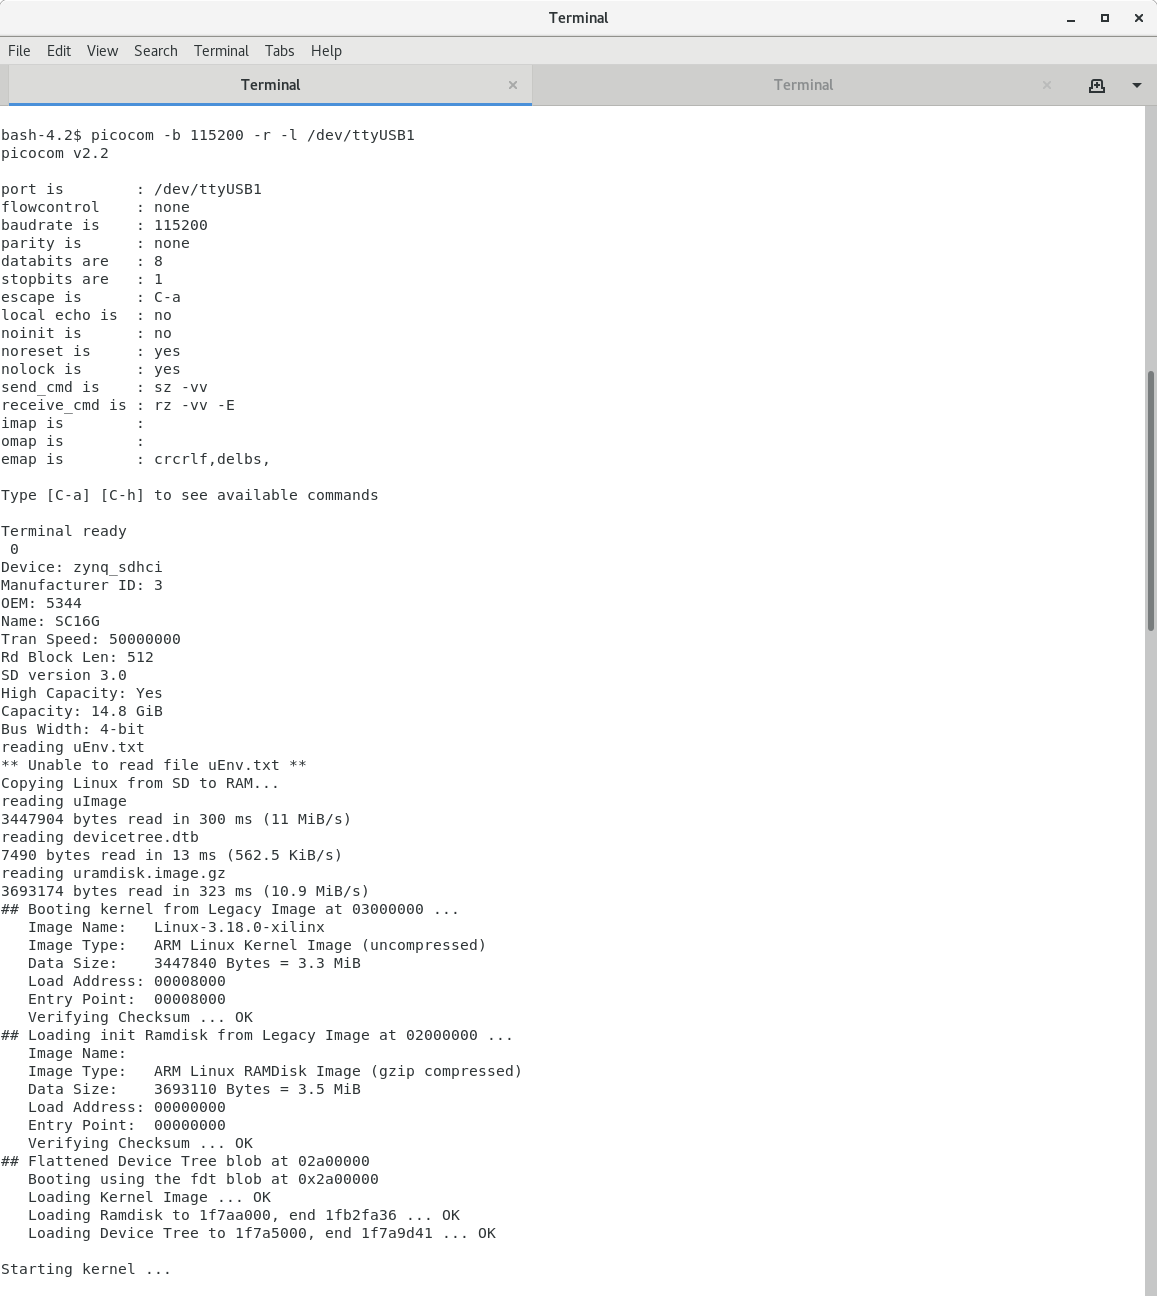
\includegraphics[width=0.85\textwidth]{boot_1.png}
    \caption{Booting Linux on ZYBO Z7-10 Picocom output 1/4.}
\end{figure}

\newpage

\begin{figure}[h!]
    \centering
    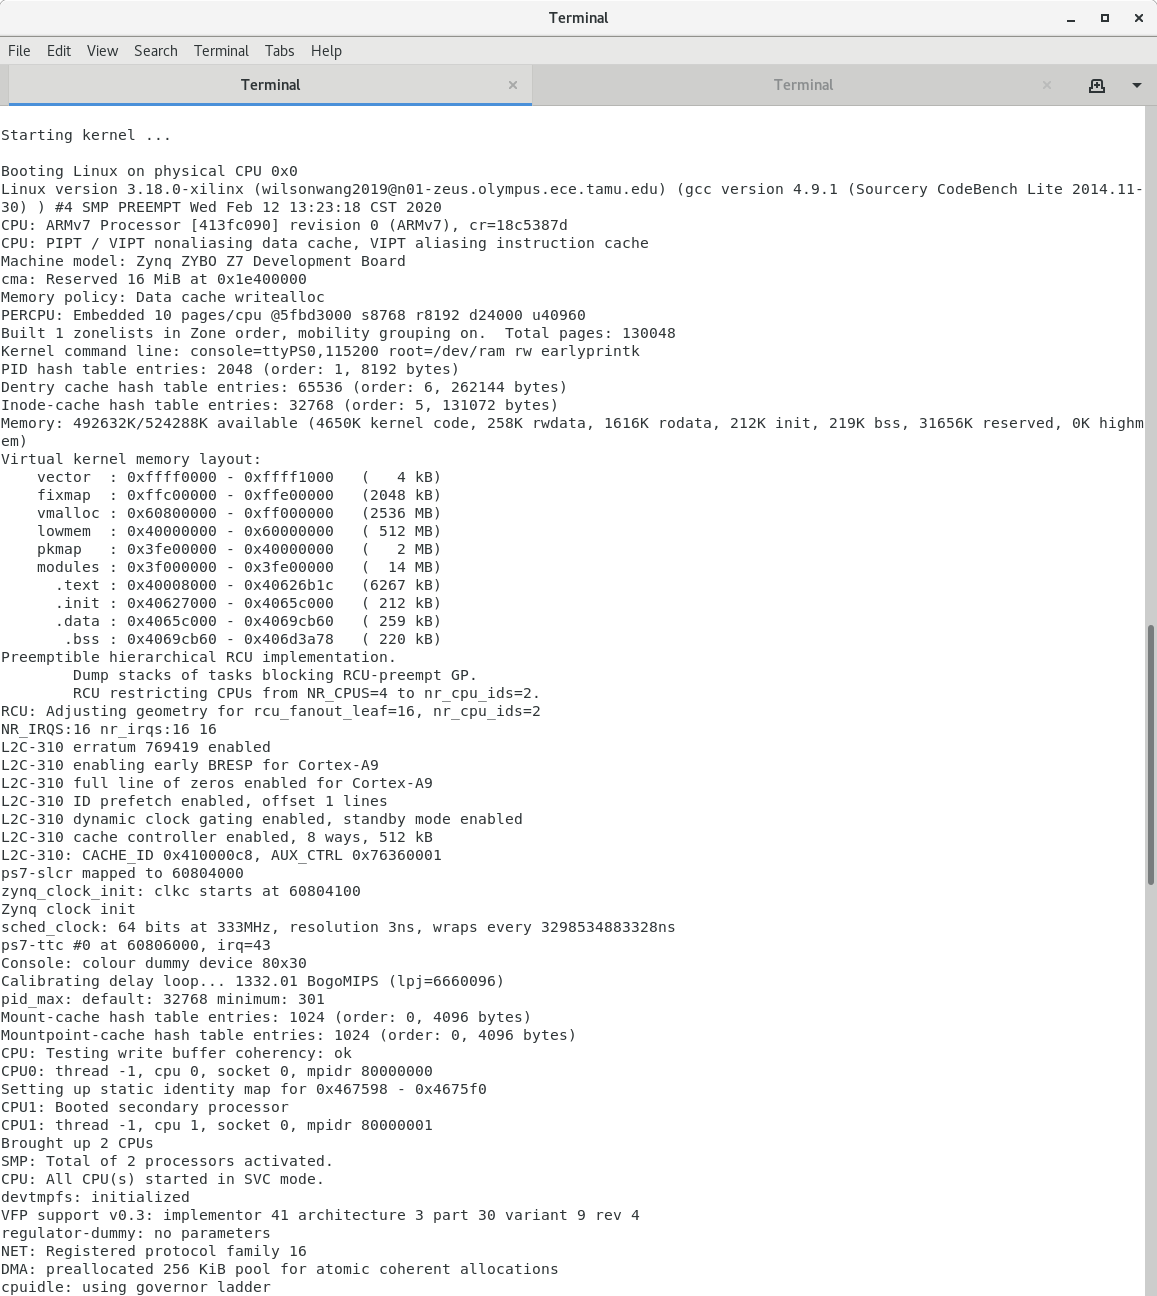
\includegraphics[width=\textwidth]{boot_2.png}
    \caption{Booting Linux on ZYBO Z7-10 Picocom output 2/4.}
\end{figure}

\newpage

\begin{figure}[h!]
    \centering
    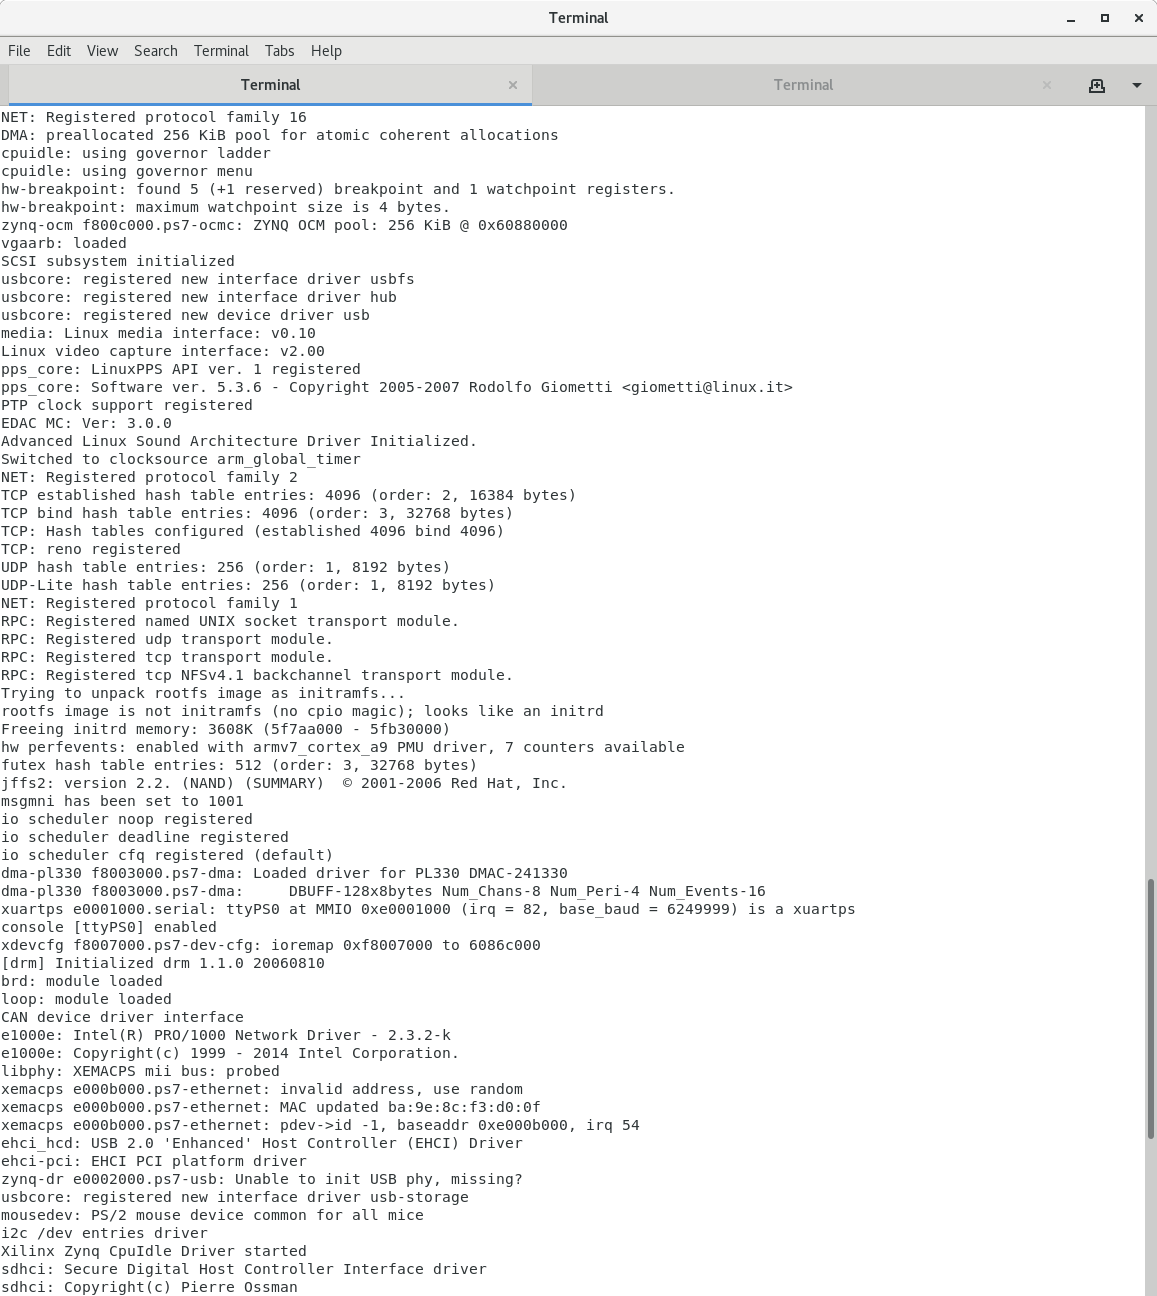
\includegraphics[width=\textwidth]{boot_3.png}
    \caption{Booting Linux on ZYBO Z7-10 Picocom output 3/4.}
\end{figure}

\newpage

\begin{figure}[h!]
    \centering
    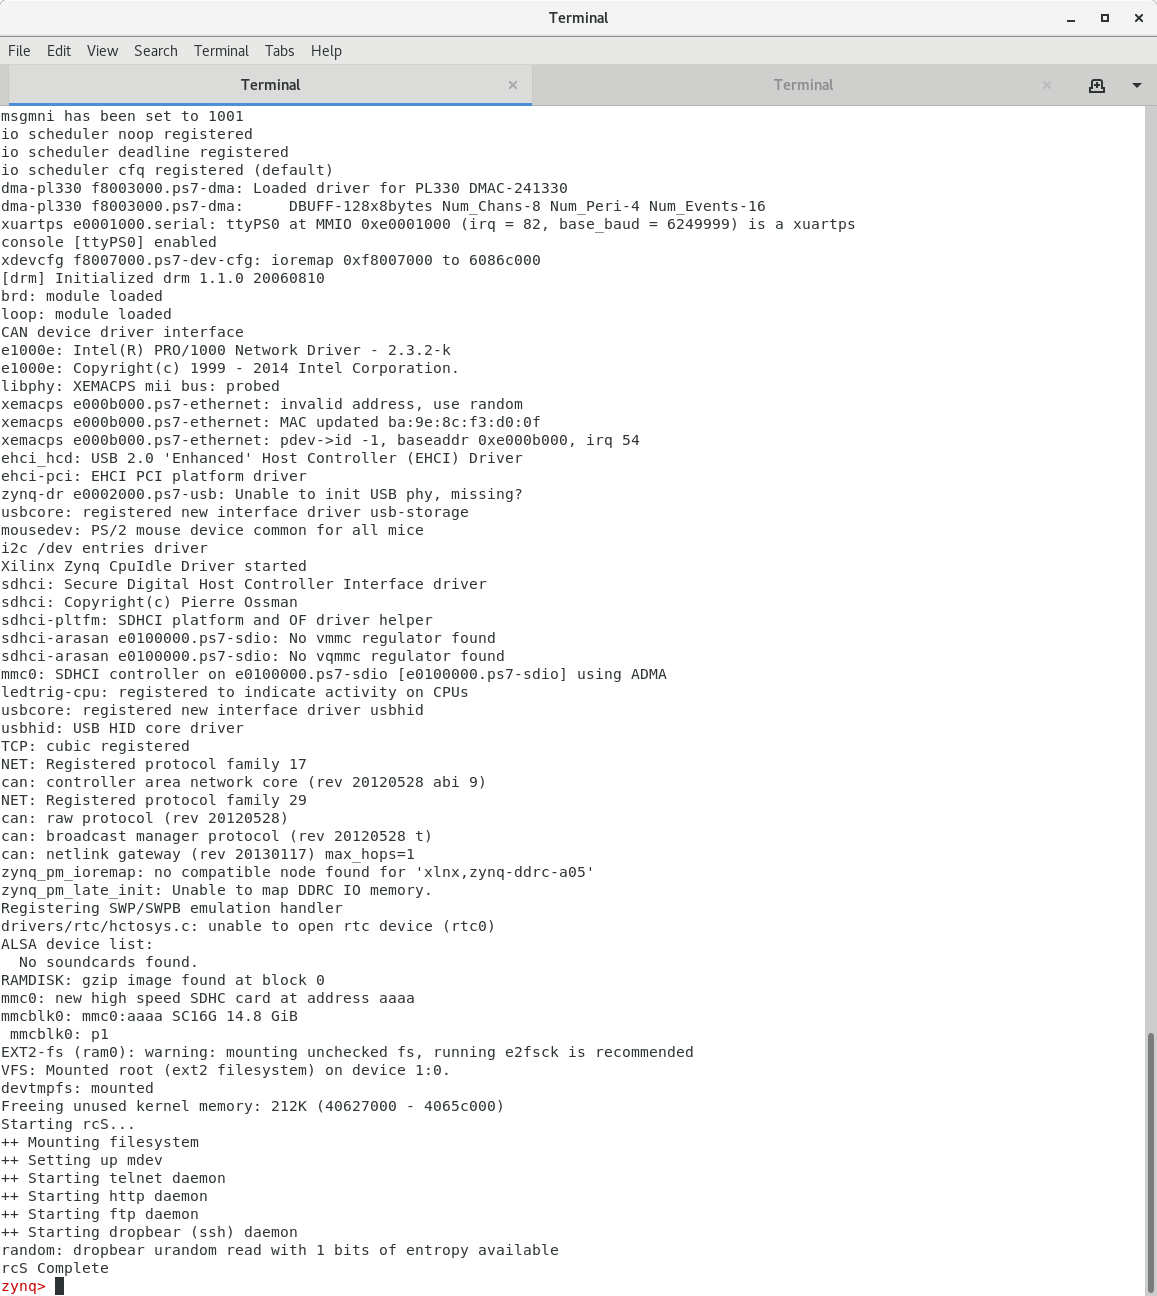
\includegraphics[width=\textwidth]{boot_4.png}
    \caption{Booting Linux on ZYBO Z7-10 Picocom output 4/4.}
\end{figure}

The FPGA programming done LED light should be on after a successful boot.

\newpage

\part{Conclusion}

The board successfully boots Linux with programmable logic configured when power on. All files, including the boot loader, the Linux system image and the file system have been properly configured and compiled. A computer system cannot boot the operating system directly, instead, a loader program is needed to guide the system to start basic functionalities such as hardware driver in order to be able to load the operating system. A loader program, under the context of lab 4, is divided into different stages. A first stage loader prepares the processing core and configure the programmable logic. A second loader then prepares the initializing of the Linux kernel. In order to be able to process and store files, a file system is needed. To include our customized IP, a device tree is configured.

\textbf{Q: Compared to lab 3, the lab 4 microprocessor system shown in Figure 1 has 512 MB of SDRAM. However, our system still includes a small amount of local memory. What is the function of the local memory? Does this ``local memory'' exist on a standard motherboard? If so, where?}

A: The local memory acts as a cache for high speed data exchange and volatile data storage. In the case that the data are so large and cannot fit in the local memory, DDR memory will be used. However, DDR memory is slow and the local memory acts as a buffer to compensate the speed mismatch between the chip, including the ARM processor and the programmable logic unit, and DDR memory. 

On a standard motherboard, memory chips may exist such as the NVRAM and the BOIS for storing configurations and handle basic I/O operations when no operating system is loaded. However, such chips are not volatile memories and are not the same type of memory as the local memory found in our system.

CPUs found on modern motherboards have high-speed caches that have the same functionality as the local memory does in our system. Commonly CPU caches are divided into L1, L2 and L3, each with different speeds and sizes.

\textbf{Q: After your Linux system boots, navigate through the various directories. Determine which of these directories are writable. (Note that the man page for ``ls'' may be helpful). Test the permissions by typing ``touch $<$filename$>$'' in each of the directories. If the file, $<$filename$>$, is created, that directory is writable. Suppose you are able to create a file in one of these directories. What happens to this file when you restart the ZYBO Z7-10 board? Why?}

A: Permissions to write files are tested by running \verb|ls -al| in Picocom. The console output is in figure \ref{ls_result}.

\begin{figure}[ht]
    \centering
    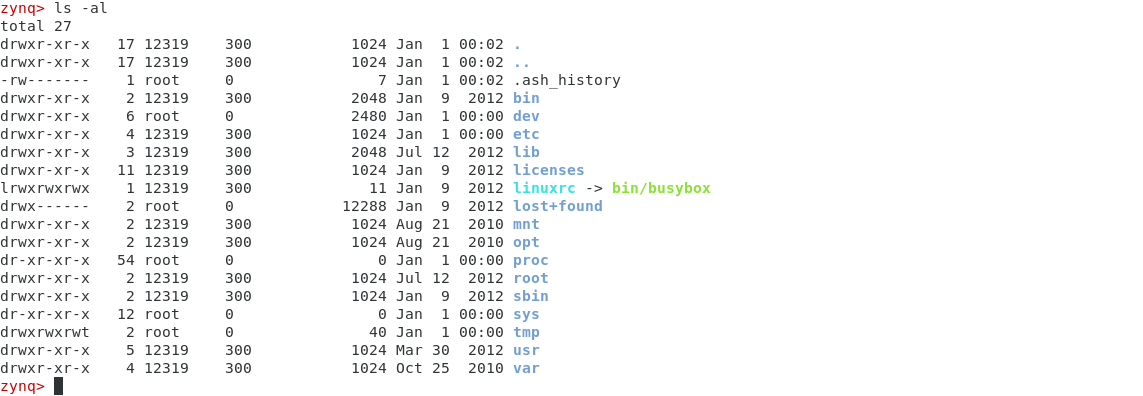
\includegraphics[width=\textwidth]{ls.png}
    \caption{ls -al output in Picocom.}
    \label{ls_result}
\end{figure}

After using \verb|cd <directory>| to each directory and run \verb|touch hello.txt|, I found that any directory with \verb|drwxr-xr-x| permission is writable. Directories with different permissions are described in table \ref{permission_table}. Tests are carried out without using \verb|sudo|.

\newpage

\begin{table}[h!]
\centering
\begin{tabular}{@{}lcc@{}}
\toprule
Name                              & Permission & Writable? \\ \midrule
.ash\_history                     & -rw- - - - - - - & Not a directory          \\ \midrule
linuxrc $\rightarrow$ bin/busybox & lrwxrwxrwx & No        \\ \midrule
lost + found                      & drwx- - - - - - & Yes          \\ \midrule
proc                              & dr-xr-xr-x & No          \\ \midrule
sys                               & dr-xr-xr-x & No          \\ \midrule
tmp                               & drwxrwxrwt & Yes       \\ \bottomrule
\end{tabular}
\caption{Linux directories whose permission is not drwxr-xr-x.}
\label{permission_table}
\end{table}

After rebooting the board, all changes made to the file system and directories are list. For instance, the \textbf{.txt} files created disappear. This is because the changes are inside RAM and not written to secondary memory, i.e. the micro-SD card. RAM is volatile and after rebooting, its content is lost.

\textbf{Q: If you were to add another peripheral to your system after compiling the kernel, which of the above steps would you have to repeat? Why?}

A: If one were to add one peripheral I/O, such as USB or Ethernet, one needs to repeat the step for \textbf{creating hardware layout} and creating \textbf{BOOT.bin}. If one were to add IP to the block design, one needs to repeat the step for \textbf{creating hardware layout}, creating \textbf{BOOT.bin} and \textbf{compiling the device tree}. Peripheral changes are related to hardware. Software such as ramdisk or the uimage are not relevant. So only repeating the steps related to hardware is sufficient.

\end{document}
